\documentclass{scrartcl}
\usepackage[utf8]{inputenc} % Unicode support (Umlauts etc.)
\usepackage{hyperref} % Add a link to your document
\usepackage{graphicx} % Add pictures to your document
\usepackage{listings} % Source code formatting and highlighting
\usepackage[top=75px, bottom=75px, left=85px, right=85px]{geometry} % Change page borders
\usepackage{graphicx}
\usepackage{mathtools}


\begin{document}

\title{Computational Intelligence:
\\Report assignment 3}
\date{\today{}}

\author{
    \begin{tabular}{l r}
    	\\Tjitte de Jong - 4172930
	\\Boris Mulder - 4100794
        \\Max Spanoghe - 4331834
            \end{tabular}
  }
  
\maketitle \thispagestyle{empty} \pagebreak
  
\section{ANT PREPARATION: OBSERVE THE PROBLEM}
  Here we will answer the questions about the observation of the problem.
  
\subsection{}
First of all it could be possible that the ant is in a very big room. This would be difficult because it is hard to find the exit and the ant can make an unnecessary turns which can lead to a very long path.
Secondly, it could happen that the ant gets in a dead end and needs to go back all the way to a previous choice point.

\subsection{}
The ants drop Pheromones to let the other ants know the popularity of a certain path. The amount of pheromone dropped is dependent on how long the path is that he took. The equation which determines the amount of pheromones par path is: \\
$Pheromone_on_link_i = \frac{n}{Path length}$
The parameter n is the estimated pathlength.

\subsection{}
 The evaporation of a link i is is actually the Pheromones that are getting away from that link. For example:\\
 evaporation constant $\alpha$ = 0.1;\\
 Pheromones on link in iteration i = p ;\\
 Then \\
 Pheromones on link in next iteration = (1-$\alpha$)*p;\\
 The evaporation is very handy to get a more quick convergence to a certain path. If a path it not chosen the links on that path get less pheromones after each iteration. In this way, the chances that ants take a path that is not very popular decreases much faster. Each iteration the pheromones go down relatively because they don't take the path, but also because of the evaporation.
 
 \section{IMPLEMENTING SWARM INTELLIGENCE}
 Here we will answer the questions about the actual implementation.
 
 \subsection{}
 The following parameters are used in the basic version of our system:\\
 $ iterations = 30; $\\
 $ ants = 3; $ \\
 $ pher = estimate of route length; $\\
 $ evaporation constant = 0.9;we want fast convergence) $\\ 
converge criterion is when the first ant in 5 iterations take the same path.\\
\pagebreak

pseudo-code:\\
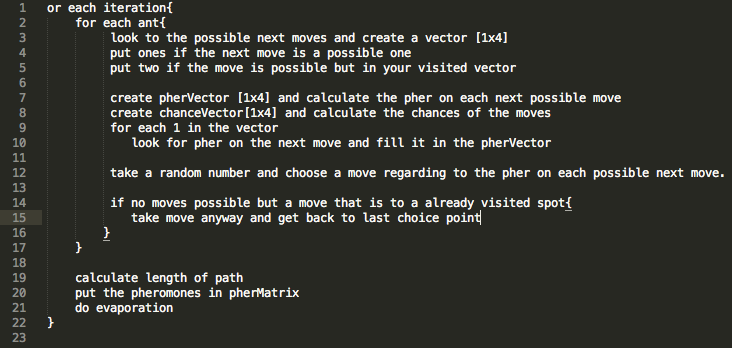
\includegraphics[width=1\textwidth]{pseudo.PNG}

\pagebreak
\section{UPGRADING YOUR ANTS WITH INTELLIGENCE}
Here we will answer the questions about how to upgrade the intelligence of the ants.

\subsection{}
Especially for the big rooms we have found a better solution than the normal maze solving algorithm we had before. The way it works is pretty good and still easy enough to implement quickly. If the ant enters a big room we do a check. If the ant has four possible next moves he will do this as long as he has 4 next possible moves:\par
take a direction just based on the normal solution and forbid him to take the opposite direction again.
In this way, he will move but never have loops in a big room. It stops when he hits a wall, bounce and will do it again eventually. This method prevent the ant of doing stupid loops in a big room. For example, if you are in a big room and you cannot see the actual walls. What one would do is start walking until he sees a wall, but never move back until you have found one, since you know there is nothing there but open space. Once you see a wall and you see there is no exit, you will bounce and start walking in the other direction again or just follow the walls. This is actually what this algorithm does so it actually works like a real person would solve the maze big rooms.

\section{PARAMETER OPTIMIZATION}
\includegraphics[width=1\textwidth]{.PNG}
\includegraphics[width=1\textwidth]{.PNG}
\includegraphics[width=1\textwidth]{.PNG}
\pagebreak
\section{PART 2: THE TRAVELING ROBOT PROBLEM}

\begin{figure}[h!]
  \caption{Plot of different sets of parameters and their convergence for the easy maze.}
  \centering
    \includegraphics[width=0.5\textwidth]{}
    \label{figure1}
\end{figure}

\begin{figure}[h!]
  \caption{Plot of different sets of parameters and their convergence for the easy maze.}
  \centering
    \includegraphics[width=0.5\textwidth]{gull}
    \label{fiure2}
\end{figure}

\begin{figure}[h!]
  \caption{Plot of different sets of parameters and their convergence for the easy maze.}
  \centering
    \includegraphics[width=0.5\textwidth]{gull}
    \label{figure3}
\end{figure}





 
 
 
 	
		 
		 
		
 
\end{document}